\documentclass{standalone}
\usepackage{color}
\usepackage{tikz}
\usepackage{animate}
\usepackage{calc}
\usetikzlibrary{arrows}
\usetikzlibrary{calc}
\usetikzlibrary{backgrounds}
\usetikzlibrary{shapes.arrows}

\begin{document}

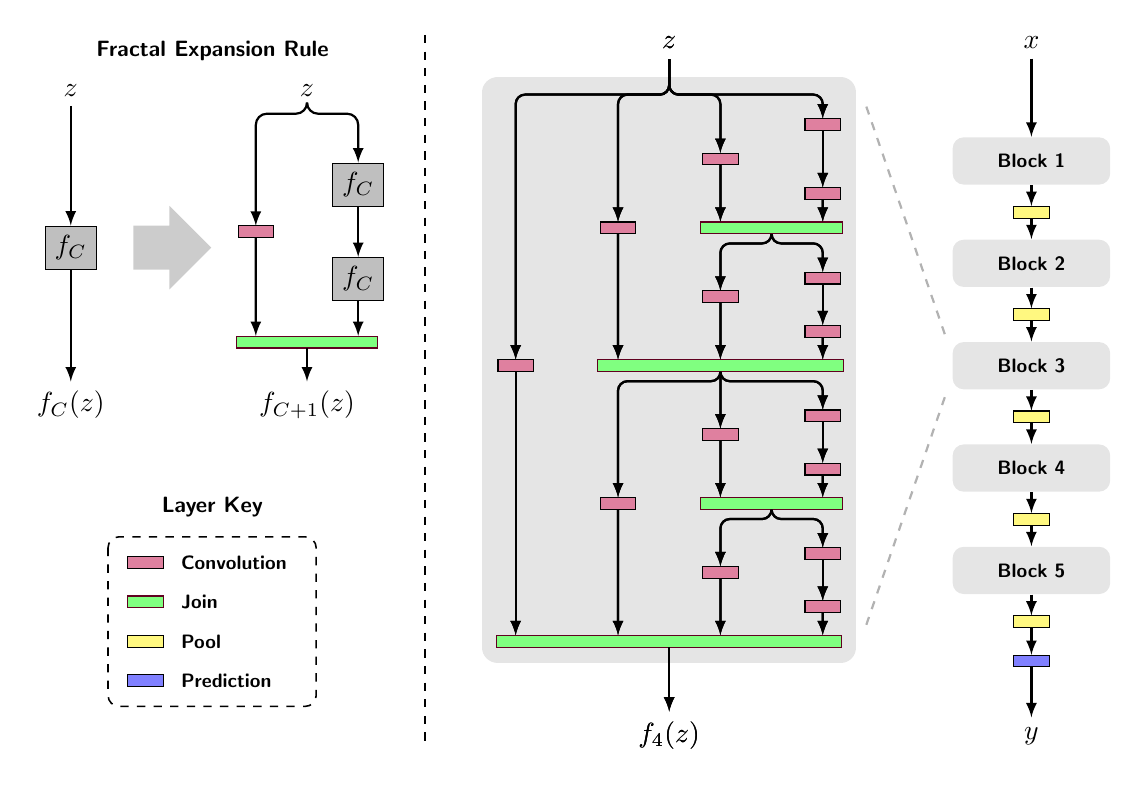
\begin{tikzpicture}[->,>=latex,auto,node distance=3cm,transform shape,
 thick,main node/.style={circle,draw,font=\sffamily\Large\bfseries}]
\def\blockheight{7.0}
\def\layerwidth{0.3}
\def\layerheight{0.04}
\def\columnwidth{1.3}
\def\one{5}

\def\blocks{1}
\def\columns{4}

\def\arrowbuf{0.12}
\tikzstyle{conv}=[rectangle,draw,thick,fill=purple!50,thin,minimum width=1.5cm,minimum height=0.5cm,scale=0.3]
\tikzstyle{pool}=[rectangle,draw,thick,fill=yellow!50,thin,minimum width=1.5cm,minimum height=0.5cm,scale=0.3]
\tikzstyle{dense}=[rectangle,draw,thick,fill=blue!50,thin,minimum width=1.5cm,minimum height=0.5cm,scale=0.3]
\tikzstyle{func}=[rectangle,draw,thick,fill=gray!50,thin,scale=1.0]
\tikzstyle{joiner}=[rectangle,thick,draw,fill=green!50,draw=black!50!purple,thin,minimum width=1.5cm,minimum height=0.5cm,scale=0.3]
\tikzstyle{joiner1}=[rectangle,thick,draw,fill=green!50,draw=black!50!purple,thin,minimum width=14.6cm,minimum height=0.5cm,scale=0.3]
\tikzstyle{joiner2}=[rectangle,thick,draw,fill=green!50,draw=black!50!purple,thin,minimum width=10.4cm,minimum height=0.5cm,scale=0.3]
\tikzstyle{joiner3}=[rectangle,thick,draw,fill=green!50,draw=black!50!purple,thin,minimum width=6.0cm,minimum height=0.5cm,scale=0.3]
\tikzstyle{myround}=[rounded corners=0.12cm]
\tikzstyle{arrow}=[->,thick]

\foreach \b in {1, \blocks} {
    \node[joiner1] (joiner-\b-1-1) at (\one+\columnwidth*\columns/2, -\b*\blockheight) {};
    \foreach \j in {1, ..., 1} {
        \node[joiner2] (joiner-\b-2-\j) at (\one+\columnwidth*2.5, -\b*\blockheight +\blockheight -\blockheight/2 - \j*\blockheight/1 + \blockheight/1) {};
    }
    \foreach \j in {1, ..., 2} {
        \node[joiner3] (joiner-\b-3-\j) at (\one+\columnwidth*3, -\b*\blockheight +\blockheight -\blockheight/4 - \j*\blockheight/2 + \blockheight/2) {};
    }
    \foreach \c/\layers in {1/1, 2/2, 3/4, 4/8} {
        \def\x{\one+\c*\columnwidth - \columnwidth/2}
        \def\y{\blockheight-\b*\blockheight}
        \def\convradius{\blockheight/\layers}
        \foreach \n in {1, ..., \layers} {
            \ifthenelse{\c=4 \AND \n=3}{
                \def\yn{\y - \n*\convradius + 0.5*\convradius - 0.2}
            }{
                \ifthenelse{\c=4 \AND \n=5}{
                    \def\yn{\y - \n*\convradius + 0.5*\convradius - 0.2}
                }{
                    \ifthenelse{\c=4 \AND \n=7}{
                        \def\yn{\y - \n*\convradius + 0.5*\convradius - 0.2}
                    }{
                        \def\yn{\y - \n*\convradius + 0.5*\convradius}
                    }
                }
            }
            \def\xn{\x}
            \node[conv] (conv-\b-\c-\n) at (\xn, \yn) {};
        }

    }

    \node (entry) at (\one+\columnwidth*\columns/2, 0.6) {$z$};
    \node (below-entry) at (\one+\columnwidth*\columns/2, 0.1) {};

    \draw[arrow,myround] (entry.south) to ($(entry.south) + (0, -0.45)$) to ($(entry.south) + (+\columnwidth*1.5, -0.45)$) to  (conv-\b-4-1);
    \draw[arrow,myround] (entry.south) to ($(entry.south) + (0, -0.45)$) to ($(entry.south) + (+\columnwidth*0.5, -0.45)$) to  (conv-\b-3-1);
    \draw[arrow,myround] (entry.south) to ($(entry.south) + (0, -0.45)$) to ($(entry.south) + (-\columnwidth*0.5, -0.45)$) to  (conv-\b-2-1);
    \draw[arrow,myround] (entry.south) to ($(entry.south) + (0, -0.45)$) to ($(entry.south) + (-\columnwidth*1.5, -0.45)$) to  (conv-\b-1-1);

    \draw[arrow] (conv-\b-4-1) to (conv-\b-4-2);
    \draw[arrow] (conv-\b-4-2) to ($(joiner-\b-3-1.north) + (\columnwidth/2, 0)$);
    %\draw[arrow] ($(joiner-\b-3-1.south) + (\columnwidth/2, 0)$) to (conv-\b-4-3);
    \draw[arrow,myround] (joiner-\b-3-1.south) to ($(joiner-\b-3-1.south) + (0, -\arrowbuf)$) to ($(joiner-\b-3-1.south) + (\columnwidth/2, -\arrowbuf)$) to (conv-\b-4-3);
    \draw[arrow] (conv-\b-4-3) to (conv-\b-4-4);
    \draw[arrow] (conv-\b-4-4) to ($(joiner-\b-2-1.north) + (\columnwidth, 0)$);
    %\draw[arrow] ($(joiner-\b-2-1.south) + (\columnwidth, 0)$) to (conv-\b-4-5);
    \draw[arrow,myround] (joiner-\b-2-1.south) to ($(joiner-\b-2-1.south) + (0, -\arrowbuf)$) to ($(joiner-\b-2-1.south) + (\columnwidth, -\arrowbuf)$) to (conv-\b-4-5);
    \draw[arrow] (conv-\b-4-5) to (conv-\b-4-6);
    \draw[arrow] (conv-\b-4-6) to ($(joiner-\b-3-2.north) + (\columnwidth/2, 0)$);
    %\draw[arrow] ($(joiner-\b-3-2.south) + (\columnwidth/2, 0)$) to (conv-\b-4-7);
    \draw[arrow,myround] (joiner-\b-3-2.south) to ($(joiner-\b-3-2.south) + (0, -\arrowbuf)$) to ($(joiner-\b-3-2.south) + (\columnwidth/2, -\arrowbuf)$) to (conv-\b-4-7);
    \draw[arrow] (conv-\b-4-7) to (conv-\b-4-8);
    \draw[arrow] (conv-\b-4-8) to ($(joiner-\b-1-1.north) + (\columnwidth*1.5, 0)$);


    \draw[arrow] (conv-\b-3-1) to ($(joiner-\b-3-1.north) - (\columnwidth/2, 0)$);
    %\draw[arrow] ($(joiner-\b-3-1.south) - (\columnwidth/2, 0)$) to (conv-\b-3-2);
    \draw[arrow,myround] (joiner-\b-3-1.south) to ($(joiner-\b-3-1.south) + (0, -\arrowbuf)$)  to ($(joiner-\b-3-1.south) + (-\columnwidth/2, -\arrowbuf)$)  to (conv-\b-3-2);
    \draw[arrow] (conv-\b-3-2) to (joiner-\b-2-1);
    \draw[arrow] (joiner-\b-2-1) to (conv-\b-3-3);
    \draw[arrow] (conv-\b-3-3) to ($(joiner-\b-3-2.north) - (\columnwidth/2, 0)$);
    %\draw[arrow] ($(joiner-\b-3-2.south) - (\columnwidth/2, 0)$) to (conv-\b-3-4);
    \draw[arrow,myround] (joiner-\b-3-2.south) to ($(joiner-\b-3-2.south) + (0, -\arrowbuf)$) to ($(joiner-\b-3-2.south) + (-\columnwidth/2, -\arrowbuf)$) to (conv-\b-3-4);
    \draw[arrow] (conv-\b-3-4) to ($(joiner-\b-1-1.north) + (\columnwidth*0.5, 0)$);

    \draw[arrow] (conv-\b-2-1) to ($(joiner-\b-2-1.north) - (\columnwidth, 0)$);
    %\draw[arrow] ($(joiner-\b-2-1.south) - (\columnwidth, 0)$) to (conv-\b-2-2);
    \draw[arrow,myround] (joiner-\b-2-1.south) to ($(joiner-\b-2-1.south) + (0, -\arrowbuf)$) to ($(joiner-\b-2-1.south) + (-\columnwidth, -\arrowbuf)$) to (conv-\b-2-2);
    \draw[arrow] (conv-\b-2-2) to ($(joiner-\b-1-1.north) + (-\columnwidth*0.5, 0)$);

    \draw[arrow] (conv-\b-1-1) to ($(joiner-\b-1-1.north) - (\columnwidth*1.5, 0)$);

    \node (exit) at (\one+\columnwidth*\columns/2, -\blockheight-1.2) {$f_4(z)$};

    \draw[arrow] (joiner-\b-1-1) to  (exit);
}

\begin{pgfonlayer}{background}
\filldraw [line width=4mm,join=round,black!10]
  (below-entry.south -| conv-1-4-1.east) rectangle (joiner-1-1-1.south -| conv-1-1-1.west);
\end{pgfonlayer}

\def\two{\one+\columnwidth*\columns + 2}
\def\betweenblocks{1.3}

\foreach \b in {1, ..., 5} {
    \node[rounded corners,black,fill=black!10,join=round,minimum width=2.0cm,minimum height=0.6cm] (block-\b) at (\two, -\blockheight/2 -\b*\betweenblocks + 3*\betweenblocks) {\scriptsize{\textsf{\textbf{Block \b}}}};
    \node[pool] (pool-\b) at (\two, -\blockheight/2 -\b*\betweenblocks + 2.5*\betweenblocks) {};
    %\node[anchor=west] at ($(pool-\b.east) + (0.1, 0)$) {\textsf{\textbf{\scriptsize{$/$2}}}};
}

\node[dense] (dense) at ($(pool-5) + (0, -0.5)$) {};

\node[] (x) at (\two, 0.6) {$x$};
\node[] (y) at (\two,  -\blockheight-1.2) {$y$};
\draw[arrow] (x) to (block-1);
\draw[arrow] (block-1) to (pool-1);
\draw[arrow] (pool-1) to (block-2);
\draw[arrow] (block-2) to (pool-2);
\draw[arrow] (pool-2) to (block-3);
\draw[arrow] (block-3) to (pool-3);
\draw[arrow] (pool-3) to (block-4);
\draw[arrow] (block-4) to (pool-4);
\draw[arrow] (pool-4) to (block-5);
\draw[arrow] (block-5) to (pool-5);
\draw[arrow] (pool-5) to (dense);
\draw[arrow] (dense) to (y);

\draw[-,dashed,thick,black!30] (\two - 1.1, -\blockheight/2 + 0.4) -- (\two - 2.1, -\blockheight/2 + 3.3);
\draw[-,dashed,thick,black!30] (\two - 1.1, -\blockheight/2 - 0.4) -- (\two - 2.1, -\blockheight/2 - 3.3);

\def\three{0}
\def\lx{\three + 0.7 + 0.25}
\def\ly{-6}
\def\betweenlegends{0.5}

\def\leftcenter{\dividerx - 2.95}
\def\dividerx{\one-0.5}

\draw[-,dashed,thick,black] (\dividerx, 0.7) -- (\dividerx, -8.3);

\node[] (text-depth-expansion) at (\leftcenter+0.25, 0.5) {\textsf{\textbf{\footnotesize{Fractal Expansion Rule}}}};
\node[] (text-layer-guide) at (\leftcenter+0.25, \ly+0.7) {\textsf{\textbf{\footnotesize{Layer Key}}}};

\node[conv] (legend-conv) at (\lx, \ly) {};
\node[anchor=west] (legend-conv-text) at ($(legend-conv.east) + (0.1, 0)$) {\textsf{\textbf{\scriptsize{Convolution}}}};

\node[joiner] (legend-joiner) at (\lx, \ly-\betweenlegends) {};
\node[anchor=west] at ($(legend-joiner.east) + (0.1, 0)$) {\textsf{\textbf{\scriptsize{Join}}}};

\node[pool] (legend-pool) at (\lx, \ly-2*\betweenlegends) {};
\node[anchor=west] (legend-pool-text) at ($(legend-pool.east) + (0.1, 0)$) {\textsf{\textbf{\scriptsize{Pool}}}};

\node[dense] (legend-dense) at (\lx, \ly-3*\betweenlegends) {};
\node[anchor=west] (legend-dense-text) at ($(legend-dense.east) + (0.1, 0)$) {\textsf{\textbf{\scriptsize{Prediction}}}};

\def\buf{0.25}
\begin{pgfonlayer}{background}
\draw [line width=0.2mm,dashed,rounded corners]
  ($(legend-conv.north -| legend-conv.west) + (-\buf, \buf)$) rectangle ($(legend-dense.south -| legend-conv-text.east) + (\buf, -\buf)$);
\end{pgfonlayer}


\def\ex{\three}
\def\ey{0.0}
\def\exb{\three + 3.0}
\def\eheight{4.0}
\def\eradius{\columnwidth/2}

\node[] (ex-1) at (\ex, \ey) {$z$};
\node[func] (ef-1) at (\ex,\ey - 0.5*\eheight) {$f_{C}$};
\node[] (ey-1) at (\ex, \ey-\eheight) {$f_{C}(z)$};
\draw[arrow] (ex-1) to (ef-1);
\draw[arrow] (ef-1) to (ey-1);

\node[] (ex-2) at (\exb, \ey) {$z$};
\node[conv] (econv) at (\exb - \eradius,\ey - 0.45*\eheight) {};
\node[func] (ef-2-1) at (\exb + \eradius,\ey - 0.3*\eheight) {$f_{C}$};
\node[func] (ef-2-2) at (\exb + \eradius,\ey - 0.6*\eheight) {$f_{C}$};
\node[joiner3] (ejoin) at (\exb,\ey - 0.8*\eheight) {};
\node[] (ey-2) at (\exb, \ey-\eheight) {$f_{C+1}(z)$};

\draw[arrow,rounded corners] (ex-2) to ($(ex-2) + (0, -0.3)$) to ($(ex-2) + (\eradius, -0.3)$) to (ef-2-1);
\draw[arrow,rounded corners] (ex-2) to ($(ex-2) + (0, -0.3)$) to ($(ex-2) + (-\eradius, -0.3)$) to (econv);
\draw[arrow] (ef-2-1) to (ef-2-2);
\draw[arrow] (econv) to ($(ejoin.north) + (-\eradius, 0)$);
\draw[arrow] (ef-2-2) to ($(ejoin.north) + (+\eradius, 0)$);
\draw[arrow] (ejoin.south) to (ey-2);

\node[single arrow,rotate=0,fill=black!20] at (\exb - 1.85, \ey - 0.5*\eheight) {\phantom{hej}};

\end{tikzpicture}

\end{document}
